
\documentclass[runningheads,a4paper]{llncs}

\let\proof\relax
\let\endproof\relax

\usepackage{amssymb}
\setcounter{tocdepth}{3}
\usepackage{graphicx}
\usepackage{subfig}
\usepackage{amsthm}
\usepackage{mathtools}
\usepackage{url}
\newcommand{\keywords}[1]{\par\addvspace\baselineskip
\noindent\keywordname\enspace\ignorespaces#1}
\usepackage{pifont}
\usepackage[utf8]{inputenc}
\inputencoding{utf8}

\begin{document}

\mainmatter

\title{Deadlocks as Runtime Exceptions}
\titlerunning{Deadlocks as Runtime Exceptions}

\author{Rafael Brandao Lobo%
\and Fernando Jose Castor de Lima Filho}

\authorrunning{Deadlocks as Runtime Exceptions}

\institute{Center of Informatics, Federal\\
University of Pernambuco, Brazil\\
\{rbl,castor\}@cin.ufpe.br\\
\url{http://www.cin.ufpe.br/}}

\toctitle{Deadlocks as Runtime Exceptions}
\tocauthor{Deadlocks as Runtime Exceptions}
\maketitle

\begin{abstract}
\dots
\keywords{\dots}
\end{abstract}
\chapter{Introduction}

Real-world applications use concurrency to parallelize computation in multiple threads or processes, taking more advantage of multicore processors.
However concurrenct code is difficult to write correctly, as it is well documented in \cite{lu}. In a concurrent code, for example, a developer must
take in consideration all possible interleaves that multiple threads in the running code can take which is simply not feasible.
When multiple threads access concurrently a certain memory position, data races may occur.
One way to solve this problem is to first identify parts of the code that should not allow threads to run simultaneously -- they are
called critical sections -- and then protect them by using locks. 

Locks are used to avoid data races in concurrent code. When a thread acquires a certain lock, no other thread can acquire the same lock.
Any thread that attempt to acquire that lock will be blocked until that resource is released. Once that thread finishes to execute critical code,
it should release that lock so other threads would be unblocked afterwards.

Unfortunately locks cannot be easily composed in the code and a very common bug caused by composing locks in unexpected ways is called deadlock.
A deadlock manifests when threads are waiting each other in a cycle, each one holding locks that other thread is trying to acquire.

Suppose a thread X acquires a lock A and then tries to acquire a lock B. Given the nature of parallelism, another thread Y simultaneously acquires
a lock B and then tries to acquire lock A. Since thread X is blocked waiting for lock B to be released and thread Y which owns lock B is blocked
waiting for thread X to release lock A, both will never finish waiting, thus creating a deadlock. When a deadlock happens, a program fail
to make progress without notice to users and developers, making harder to identify the problem.

Deadlocks can be avoided if locks are acquired in any order, as long as the other threads follows that particular order. For example, if both thread X
and thread Y always acquired locks A and B in this order, then no deadlock could ever occur because there's no waiting relationship cycle between them. 
Some existing techniques to avoid deadlock require to impose a global order on locks and check whether this order is ever violated when the locks are acquired \cite{marino},
but this approach is not practical for real world software because most of the time the code that acquires the first lock is unaware of wh.

There are two main types of deadlocks: resource deadlocks and communication deadlocks \cite{singhal} \cite{knapp}. Resource deadlocks are illustrated in the previous
example, where threads wait for resources to become available. Communication deadlocks happens when threads are blocked waiting messages, so messages are the resources
for which threads wait. In this work, as other studies did before \cite{mcsdk} \cite{magicfuzzer}, our focus will be on resource deadlocks and from now on and whenever the term \emph{deadlock} is used by itself we will be referring to resource deadlocks unless mentioned otherwise.

Over the time, many studies tried to solve deadlock by detecting them in many different ways which can be made by either static analysis, dynamic analysis, or a mix of them. Static analysis leverage deadlock existence by reading the source code and estimating whether a deadlock would be possible with that code without actually running it. In counter part, dynamic analysis dynamically add extra code in the original source and possibly detect real deadlocks during execution. But each one of those techniques
have its own advantages and disadvantages and they complement one another.

In this study, however, we are focusing on solving deadlocks differently. We believe deadlocks should not fail silently but instead they should be handled as exceptions in programming languages. Rather than trying to detect them when explicitly requested for a deadlock analysis, programs should instead be written in such a way that they can either handle the deadlock when it happens by deploying some custom deadlock recovery logic or just show the error in the output in order to ease finding bugs and solving them later.

There are some programming languages such as Haskell and Go that already contain some kind of deadlock exception for very particular cases. In this study, the proposed deadlock exception was focused on what we've found out to be the most common type of deadlock: the classical deadlock illustrated in the previous example where only two threads are involved and they're waiting circularly for two resources.

\section{Summary of Goals}

In this work we have the main goal to show how deadlock detection between two threads and two locks can be implemented with very low runtime overhead and evaluate the impact of deadlock exceptions on the efficiency of identifying deadlocks in software by running an empirical study with students. With this contribution, we seek to understand the benefits of such exceptions in programming languages and also offer a lightweight implementation of deadlock exceptions that can seamlessly run on top of Java OpenJDK.

\section{Outline}

The remainder of this work will be organized as follows:

\begin{itemize}
  \item Chapter 2 discuss the basic concepts of deadlock exceptions, highlighting previous studies and terms that are necessary to understand before proceeding to the next chapters.
  \item Chapter 3 presents our study on bug reports in open source projects, focusing on deadlock bugs and identifying some of its characteristics.
  \item Chapter 4 shows our deadlock detection algorithm in details, presenting a sketch of a formal proof, what changes were done to Java's ReentrantLock and a quick performance evaluation.
  \item Chapter 5 discuss the empiric evaluation we did to measure efficiency of deadlock exceptions on identifying bugs in software.
  \item Chapter 6 presents the contributions of this work, discusses some related and future work, and presents our main conclusions.
  \item Appendix A shows the code used to calculate the size of sample we've used in Chapter 3.
  \item Appendix B shows the code used to analyse the data collected in Chapter 3.
  \item Appendix C shows the code used to collect the data from different repositories used in Chapter 3.
  \item Appendix D shows Java's ReentrantLock pseudocode cited in Chapter 4.
  \item Appendix E shows R instructions to evaluate time used in Chapter 5.
  \item Appendix F shows input for R script used to analyse time in Chapter 5.
\end{itemize}




\section{Bug Reports Study}\label{bugs}

Attempting to generalize deadlock detection at runtime does not seem feasible from a performance viewpoint, since existing dynamic analyses take considerable time~\cite{magicfuzzer}. But previous bug reports study~\cite{lu} found that 30 out of 31 deadlock bug reports involved at most two resources. We suspected TTTL deadlocks were more common in real world systems than more complex deadlocks, so we investigated this further. This section presents the results of this investigation.

\subsection{Sample Collection}

We've chosen three open source projects which used Java as main programming language and made use of concurrent programming: Lucene\footnote{Lucene: http://lucene.apache.org/}, Eclipse\footnote{Eclipse: https://eclipse.org/} and OpenJDK\footnote{OpenJDK: http://openjdk.java.net/}.

Lucene is a text search engine library that can be used along many applications, where concurrent programming was used to deliver high performance. Eclipse is one of the most popular IDE for java developers. OpenJDK is an open-source implementation of the Java Platform. These three projects share a few similarities: they're written in Java; they have vast inventory of bug reports on their repositories and publicly available tools to search for bug reports; and lastly, they share a software development culture of reviews inside bug reports by discussing solutions to fix the problem. In particular, this last characteristic was very important to allows us to analyze bug reports and infer their classification with confidence.

We have initially searched in each repository for the keyword \emph{deadlock}, and we've collected 541 bug reports in total.
Each project had a different bug repository, so we've changed slightly the query parameters to find relevant bug reports.
In Lucene, we've searched for bugs matching the word "deadlock" anywhere in the bug report (i.e. in summary or in comments), related to module "lucene-core" where issue type was set as "bug" and whose status was set as "closed"; from this search, we've found 27 bugs~\footnote{Lucene bug reports: http://goo.gl/DhVI3t}.
In Eclipse, we've searched for the word "deadlock" in summary, where resolution was set as "fixed" and whose status was set as "resolved"; from this search, we've found 406 bugs~\footnote{Eclipse bug reports: http://goo.gl/qQnrEm}.
In OpenJDK, we've searched for bugs with the word "deadlock" inside the summary, related to its module named "JDK", where issue type was "bug", resolution was "fixed" and status was "resolved"; finally, from this search, we've found 108 bugs~\footnote{OpenJDK bug reports: http://goo.gl/xYFfsO}.
We then proceeded to calculate the sample size that would allow us to have 95\% of confidence level and 5\% sampling error with 50\% of response distribution, which resulted in 225 bugs.
Thus we created a random sample\footnote{Bug reports sample: http://goo.gl/zNsIGz} of that size to analyze further.

\subsection{Data Labeling}

We've merged all bug reports of our random sample in one single table, where each row represented a different bug report and each column represents an attribute that we were interested.
The first attribute was the name of the bug. Each name was composed by a prefix that could be either \emph{LUCENE}, \emph{ECLIPSE} or \emph{JDK}, followed by the bug number on their own repository.
The second attribute was the category: a character that could be either "A", "B", "C" or "D", added by us after going through that particular bug report with our manual inspections.
Other fields such as \emph{type}, \emph{number of threads}, \emph{number of resources} and \emph{notes} will be detailed shortly. Although we collected additional fields such as \emph{time} and \emph{comments} and made available in the final version of this table\footnote{Bug reports sample table: http://goo.gl/zNsIGz}, we did not use them for the analysis of this work.

\subsubsection{Category.}

This is one of the most important fields, as we want to be able to identify what kind of deadlock this bug represents, or if it's not a real deadlock. We have four different values for this field and they must be one of the following:

\begin{itemize}
\item \emph{A:} We are confident this a resource deadlock. We should be able to provide a short explanation of how the bug occurs, which or how many threads are involved and how many locks are involved in this bug.

\item \emph{B:} We are confident this is not a resource deadlock, so it must be a communication deadlock. It might be a lost notify/signal bug. We should be able to identify if this is a lost notify/signal or have clear evidence this is not a resource deadlock (adding a note whenever possible).

\item \emph{C:} We are confident this is a false-positive for "deadlock" search. The term was used as a synonym of "hang" or "infinite loop", or to refer to another deadlock bug. In some cases, it is possible that a bug refers to another bug which was fixing a deadlock, so the initial bug may not be deadlock-related and just fix a regression for another bug (which could be deadlock-related). In other words, this is not a deadlock bug at all.

\item \emph{D:} We are not confident whether this is a resource deadlock or a communication deadlock, or even if this is a false-positive for deadlock. There's not enough information in the bug report, or the information is just inconclusive. Since we are not experts on any of these code repositories, it's hard to classify in any other category.
\end{itemize}

General guideline for classifying bugs in category A was to only assign it when there was a clear comment in the bug explaining what threads and which resources are involved or other evidences can clarify without doubt how many threads and lock resources are involved. In a few cases, the explanation was not fully clear but the attachments on the bug provided a clear thread dump report showing which threads were involved and which locks each one were holding and waiting for. When such evidence was present, we could use it to make the final decision. Similarly, bugs in category B could also be confirmed by looking into source code changes in cases where we were almost clear about its category. For example, if the patch changes areas of the code where a notifyAll is added or moved, then it serves as a strong evidence to confirm it should be indeed in category B. In other cases, it is deadlock where the first thread is holding a lock but also it is in an infinite loop waiting for others to finish while other threads are stuck waiting to acquire a lock the first thread already acquired, so we would understand it as a communication deadlock: the "message" or "signal" which the first thread have been waiting is whether the other threads have finished, but it never arrives. Luckily, category C was often easy to classify since there usually was a comment in the bug report referencing another kind of bug, using the term "deadlock" as a synonym for "hang". If a particular bug only has a comment that refers to another bug (e.g. a regression) as a deadlock bug, then the bug being investigated might not be a deadlock by itself, which would also fall into this category. Finally, category D is for all other bugs which could not be classified as either A, B or C.


\subsubsection{Number of threads/resources.}

Whenever possible, the reviewer should state the number of threads and resources involved, even if this is in the category B. If it's unknown how many resources but it is clear how many threads are involved, then only one of them should be filled and the other field should remain empty.

\subsubsection{Type.}

This field is just an annotation and it should be used to specify what kinds of resources a certain bug use. For example if there were two threads and they were in a circular deadlock, then this field should be \emph{locks/synchronized}. If explicit locks were used on both threads, then just \emph{locks} should be used, or if only synchronized blockswere involved, then just \emph{synchronized} should be present. The symbol + indicates a separation between threads, so for example "locks + wait" means that one thread holds a lock while the other (probably holding the lock) waits for a signal. Unfortunately, as this nomenclature could be confusing, the field \emph{notes} should be used to clarify and write down what was found about this bug.

\subsubsection{Notes.}

This field was encouraged to be used specially to remind other reviewers in the future of how the conclusion was made for cases where it was not straight-forward to choose the category. In these cases, it should contain the evidence found that helped the final decision to be made.

\subsection{Labeling Guidelines} 

In order to minimize error/bias on our classification and organized how the review was executed, we've created a set of guidelines that every reviewer should follow which basically describes how data should be analyzed for a certain bug, in what order, and what decisions could be made:

\begin{enumerate}
\item Look at bug title and bug main description (usually the first comment). Sometimes the reporter have an idea of how the bug occurs and which threads are involved, so this is a big help.

\item Look at further comments and see if someone understood this bug completely. Someone must have provided a reasonable explanation of how this bug occurs. If the category is already clear, then finish these steps; otherwise proceed.

\item If available, look at the patches (specially the final patch) and what changes have been made. If uncertain about this bug being in category B and the patch either moves or adds a notifyAll call, then it most likely is a category B bug. If this is not the case, then proceed.

\item If available, look at the related bugs or duplicates. It's often to find an initial bug that is unclear but which points out to a duplicate that have been largely discussed and is clear. Restart from step 1 for each of those related bugs. If a category was not assigned yet, then proceed.

\item See other attachments if available, like text files with thread dumps or stack traces. If they provide enough information to clarify which category it is, then assign a category to it, otherwise proceed.

\item Classify this bug in the category D.
\end{enumerate}

\subsection{Results Analysis}

Since we want to find how many resource deadlock bugs were TTTL deadlocks, we discard bugs in B and C category because they can't be resource deadlocks. What we have left are the bugs we could not determine its category with confidence. Thus in the worse case all bugs in category D should be resource deadlocks but none of them should be TTTL deadlocks. Worse case scenario is given by Equation~\ref{eq:worse}. In that equation, \emph{bugs(...)} returns the number of bug reports that matches all parameters. Now, if we want to look at the best case scenario, then all bugs classified in D category must also be TTTL deadlocks. In worse case, 54.7\% resource deadlocks are TTTL deadlocks, while in the best case, 95.29\% are TTTL deadlocks. In Table~\ref{tab:categ} (second column), we can see in that from all resource deadlocks we identified, 92.07\% of them are indeed TTTL deadlocks.
Another interesting finding is that 75.93\% of all deadlocks are indeed resource deadlocks.

\begin{equation}\label{eq:worse}
bugs\_ratio = \frac{ bugs(A, threads=2, resources=2) }{ bugs(A) + bugs(D) } \; .
\end{equation}

However neither the worse case nor the best case scenarios seems realistic. We believe that a more realistic scenario would be to assume that bugs in category D are distributed roughly the same way as those in categories A, B, and C. If that is the case (last column of Table~\ref{tab:categ}), out of all resource deadlocks, we estimate that 91.7\% of them would also be TTTL deadlocks. Thus TTTL deadlocks are certainly the most popular type of resource deadlocks, amounting to more than 9 out of every 10 resource deadlocks. This result makes it evident that an approach to automatically detect these deadlocks has practical value.

\begin{table}
\begin{center}
\caption{Labeled Categories and Estimations}\label{tab:categ}
\begin{tabular}{|l|l|l|}
\hline
Category & Number of Bugs & Estimated \\
\hline
A & 101 & 146 \\
A and TTTL & 93 & 134  \\
B & 32 & 46 \\
C & 23 & 33 \\
D & 69 & 0 \\
\hline
\end{tabular}
\end{center}
\end{table}

\subsection{Threats to Validity}

Although we've created a set of guidelines that all reviewers should follow with expecting to have more than one reviewer available on this research,
in reality we couldn't find more than one reviewer to execute the labeling on all bug reports due to constraints on time and resources. There is both an advantage
and a disadvantage given by this limitation. The advantage is that it is easier to guarantee that all bug reports were reviewed following the exact same set of rules
as they were all reviewed by the same person. The disadvantage, however, is that there was no second reviewer to double check if the labels
were indeed coherent to their respective bug reports.

Futhermore, one factor that might limit generalization of these findings is that we've looked at only three different open-source projects written mostly in Java.
In the real world, software is written in many different languages, where each language may have different distributions of deadlock bugs.
However, as we've implemented deadlock exceptions in Java's ReentrantLock, we focused on investigating what kind of deadlock bugs developers usually face when developing with Java.
This way we could understand whether our solution could be useful in practice.
For that purpose, we've carefully chosen popular open-source projects that represent high quality software and contain well established open source communities.
Their repositories had a rich resource of bug reports with many comments and documents that actually helped us to label each bug individually and they provided
online tools to allow us to search into their bug report archives which was essential for this study.
We believe that these projects were representative to evaluate the distribution of deadlock bugs for software written in Java.
We also suspect our findings are also true for other popular languages but we leave it open for future work.



\section{Deadlock Detection}

In this section we present the proposed approach. We extend the notion of lock by making locks responsible for both detecting TTTL deadlocks and raising exceptions whenever such deadlocks occur. In this section we present an algorithm implementing this extended notion of lock and show that our algorithm guarantees that (i) every TTTL deadlock is detected; and (ii) if an exception reporting a deadlock is raised, it must stem from the occurrence of a TTTL deadlock.

We have modified the default implementation of Java's \emph{ReentrantLock} to allow efficient runtime detection of TTTL deadlocks. It works as follows:

\begin{enumerate}
\item Each lock has a pointer to a thread, the owner of the lock, or {\tt null} when no thread owns that lock.
\item Each lock has an integer to represent its current state: 0 means the lock is free and no thread owns it (the \emph{unlocked} state), 1 means there is a thread that owns the lock (the \emph{locked} state). For simplicity, we are only interested on these two states. Nonetheless, in the implementation of \emph{ReentrantLock}, each time a thread owner acquires the same lock, this state would be incremented, and decremented each time the thread releases it.
\item Each thread has a thread-local list of pointers to locks it currently owns.
\item Each lock has a waiting queue of threads that are waiting to acquire it. Whenever a thread tries to obtain a lock when it's already acquired, the thread will add itself to the waiting queue before parking. Upon the event of releasing the lock, the owner of that lock will look for the first thread in the waiting queue and unpark it.
\item When a thread wants to acquire a lock, it will swap the current state to \emph{locked} if the current state is \emph{unlocked} atomically.
\begin{enumerate}
\item If the thread fails, it must be because the lock is already owned by some other thread, then it will add itself on the waiting queue for that lock. Finally, the thread will park.
\item Otherwise, the thread will set itself as the current owner of that lock and also add this lock to its thread-local list of pointers of locks it owns.
\end{enumerate}
\item When a thread is about to release a lock, the current owner pointer of that lock is set to {\tt null} and that lock is also removed from the thread-local list of owned locks. Finally, the lock state is changed to \emph{unlocked}.
\item Before parking, a thread will check whether there is a deadlock. When the current thread is unable to acquire its desired lock, it must be because another thread already owns it. It is possible to know who is the owner of any lock, so the current thread identifies the owner of its desired lock as the conflicting thread. Then the current thread will search on each lock of its list of owned locks if the conflicting thread is waiting for it.
\begin{enumerate}
\item If positive, then we have a circular dependency (current thread is stuck waiting for its desired lock and the conflicting thread is stuck waiting for a lock the current thread owns) and thus a deadlock exception will be raised.
\item Otherwise, the thread parks.
\end{enumerate}
\end{enumerate}

We take advantage of the current algorithm employed by \emph{ReentrantLock} and some of its guarantees listed below to avoid the need to introduce extra synchronization mechanisms or costly atomic operations during deadlock detection:
\begin{enumerate}
\item The operation of swapping the state of a lock from \emph{unlocked} to \emph{locked} must be done atomically by the thread, so only one thread can be successful at a time.
\item A thread will only park when it is guaranteed that some other thread can unpark it. Missing notifications will never happen and concurrent uses of park and unpark on the same thread will be resolved gracefully.
\item Inserts on each lock's waiting queue must be done atomically. If multiple threads concurrently attempt to insert themselves in the waiting queue on the same lock, they will both succeed eventually but the exact order of insertions is not important.
\item Once the last element in the waiting queue of a lock is read, it should be safe to read all threads in the waiting queue that arrived before the last element. Since the thread who reads the waiting queues is also the one who blocks every thread waiting on the queues, we can guarantee the only updates that could happen concurrently are new insertions at the end of each queue. However insertions in the end of the queue are not important once a last element pointer is obtained.
\end{enumerate}

%Now we show why this algorithm works:%

\begin{lemma}
The proposed protocol can always detect TTTL deadlocks.
\end{lemma}
\begin{proof}
By way of contradiction, suppose not and a TTTL deadlock occurred without it being detected.
Lets assume that threads \emph{A} and \emph{B} have both acquired locks \emph{a} and \emph{b} respectively, as follows:
\begin{equation}
write_{A}(state_{a} = locked) \rightarrow write_{A}(owner_{a} = A)
\end{equation}
\begin{equation}
write_{B}(state_{b} = locked) \rightarrow write_{B}(owner_{b} = B)
\end{equation}
In the above expressions, `$x \rightarrow y$' indicates that event $x$ happened before event $y$. Notation `$write_{B}(owner_{b} = B)$' indicates that thread $B$ wrote to variable $owner_{b}$ the value $B$. 
And now each thread will attempt to acquire the opposing lock: thread \emph{A} is trying to acquire lock \emph{b} and thread \emph{B} is trying to acquire lock \emph{a}, as follows:
\begin{equation}
read_{A}(state_{b} == locked) \rightarrow write_{A}(waiting\_queue_{b}.insert(A))
\end{equation}
\begin{equation}
read_{B}(state_{a} == locked) \rightarrow write_{B}(waiting\_queue_{a}.insert(B))
\end{equation}
The notation `$read_{A}(state_{b} == locked)$' indicates that thread $A$ read variable $state_{b}$ and obtained value $locked$.
If a TTTL deadlock happened, then both threads are now parked and all previous equations should be correct.
But before parking, each thread must check for deadlock by inspecting each lock it owns if the opposing thread is on its waiting queue.
As we initially assumed no deadlock exception has been raised, then both threads are parked and also the following equations must be correct:
\begin{equation}
read_{A}(owner_{b} == B) \rightarrow read_{A}(waiting\_queue_{a}.contains(B) == false)
\end{equation}
\begin{equation}
read_{B}(owner_{a} == A) \rightarrow read_{B}(waiting\_queue_{b}.contains(A) == false)
\end{equation}
The problem with the previous equations is that they both cannot be true simultaneously.
Before checking for deadlock, each thread must add itself on the waiting queue of its desired lock.
If it holds that the opposing thread is not in the waiting queue yet, then it must be because it did not start to check for deadlock yet, thus a contradiction.
\end{proof}

\begin{lemma}
The proposed protocol never raises a deadlock exception for a non-existent TTTL deadlock.
\end{lemma}
\begin{proof}
By way of contradiction, assume the opposite: a deadlock exception was raised and there is no real TTTL deadlock. Exactly one of the following equations must be true in order to raise a deadlock exception (if both were true at the same time, an actual deadlock would have occurred):
\begin{equation}
read_{A}(owner_{b} == B) \rightarrow read_{A}(waiting\_queue_{a}.contains(B) == true)
\end{equation}
\begin{equation}
read_{B}(owner_{a} == A) \rightarrow read_{B}(waiting\_queue_{b}.contains(A) == true)
\end{equation}
Suppose without loss of generality that the first equation is true.
It means that thread \emph{B} is waiting for lock \emph{a} and it is also the owner of lock \emph{b}.
If it is on the waiting queue, that thread is either parked already or about to park
and in both cases thread \emph{B} is going to depend on the release of lock \emph{a} to proceed.
However, as we have seem previously, thread \emph{A} at this point is also about to park and is checking for a deadlock.
If this condition holds, we have a circular dependency between threads \emph{A} and \emph{B}, a real TTTL deadlock, thus we have a contradiction.
\end{proof}

\subsection{Extension: raising exceptions in all threads}

The protocol we presented guarantees that an exception is raised in at least one of the threads involved in a deadlock. A safer approach, however, would be to have exceptions raised in both threads involved in the deadlock. In this section we describe an extension to the protocol that provides this guarantee. This does not affect how deadlock is detected but what should be done after a deadlock is detected. Thus, does not impact the correctness of the protocol. The proposed extension comprises the following:

\begin{enumerate}
\item Each lock has a list of tainted threads. This list should only be read or updated by the owner of that lock, allowing immunity from interference without any extra synchronization cost.
\item Once a deadlock is detected and the current thread is about to raise a deadlock exception, it already knows which thread is conflicting with itself and which lock that thread desires. The current thread (the owner of the desired lock) will add this conflicting thread to the tainted threads list for that lock. After that, the deadlock exception is raised.
\item When the conflicting thread is unparked and finally acquires its desired lock (it becomes the owner of that lock), then it is allowed to read the list of tainted threads. If this thread identifies itself in this list, then it must be because it was part of a deadlock before, so it removes its reference from the list and also raises a deadlock exception.
\item Every operation on the list of tainted threads of any lock (either reading or inserting values) should be followed up by some cleanup on all references to threads that are no longer running.
\end{enumerate}

That is sufficient to force both threads to raise exceptions when only one of them would raise an exception in the initial protocol. The latter only raises exception on both threads if they simultaneously reach the point where they check for deadlocks. However, for this particular case, this change introduces a different problem: dangling references.
If each thread adds their conflicting thread to the lists of tainted threads of the locks they own, 
but none of them is able to acquire their respective desired locks (as in \emph{item 3}),
both threads will leave their references behind for others to cleanup (as in \emph{item 4}).
We minimize this issue by cleaning these references as soon as any thread acquires the lock.

\subsection{Implementation}

The full version of the modified OpenJDK \emph{ReentrantLock} that implements this algorithm is available in our code repository~\cite{repo}.
In this section we will focus on what changes were done, so we will present pseudo-code to illustrate.

\medskip
\noindent
{\it Changes on ReentrantLock: keep ownedLocks list updated}
\begin{verbatim}
// This is a thread-local inside a lock.
// Each thread keeps the list of locks they own.
DEFINE_PER_THREAD(List<Lock>, ownedLocks);

// As soon as a lock is acquired or release, this function is called.
// Based on that, we call register or unregister owned lock.
void setExclusiveOwner(Thread thread) {
  owner = thread;
  if (owner == null) {
    unregisterOwnedLock();
  } else {
    registerOwnedLock();
  }
}

// These functions register or unregister the current lock
// in the thread-local list ownedLocks.
registerOwnedLock();
unregisterOwnedLock();
\end{verbatim}

Following the first part of the protocol, we must keep a list of locks each thread owns.
This list is thread-local so it's free from interference (each thread will only manage its own list).
Method calls to \emph{setExclusiveOwner} are intercepted to also update the list of owned locks accordingly as follows:
whenever the call resets the owner it means there was a release, so we unregister that lock and removes it from the list of owned locks of the current thread;
futhermore, we do the opposite when the owner is not null, as it means that the thread has owned that lock and it should update its own list of owned locks to add that particular entry.

\medskip
\noindent
{\it Changes on ReentrantLock: detect deadlock and throw exception}
\begin{verbatim}
void park() {
  Thread conflictingThread = owner;
  if (isAnyOwnedLockDesiredBy(conflictingThread)) {
    clearOwnedLocksByCurrentThread();
    throw new DeadlockException();
  }
  LockSupport.park(this);
}

// Returns true if any of the locks owned by the current thread
// contain a given thread in the waiting queue.
isAnyOwnedLockDesiredBy(Thread);

// Clear all locks in the list of owned locks by the current thread.
clearOwnedLocksByCurrentThread();
\end{verbatim}

When a thread attempts to acquire a lock and this lock is already owned, we deploy the deadlock check right before the thread actually get parked.
It starts by checking which thread is the owner of this particular lock, then the current thread checks whether there's any lock owned by itself
that is currently being waited by that conflicting thread. If positive, then we have a circular wait so we must throw a deadlock exception.
Next step is to guarantee that both threads will receive the deadlock exception.

\medskip
\noindent
{\it Changes on ReentrantLock: throw deadlock exception on both threads}
\begin{verbatim}
// Each lock will have a list of threads that are not allowed to
// acquire this lock (if it happens, throw exception).
DEFINE_PER_LOCK(List<Thread>, taintedThreads);

void park() {
  Thread conflictingThread = owner;
  List<Lock> desiredLocks =
    getOwnedLocksDesiredBy(conflictingThread);
  if (!desiredLocks.isEmpty()) {
    foreach(Lock k in desiredLocks) {
      k.taintedThreads.add(conflictingThread);
    }
    clearOwnedLocksByCurrentThread();
    throw new DeadlockException();
  }
  LockSupport.park(this);
}

// Returns a list of locks owned by the current thread where
// a particular Thread (passed as parameter) is waiting for.
getOwnedLocksDesiredBy(Thread);

// Add a check as soon as a thread acquires this lock.
// If it is marked as tainted, then throw exception.
void setExclusiveOwner(Thread thread) {
  owner = thread;
  if (owner == null) {
    unregisterOwnedLock();
  } else {
    registerOwnedLock();
    if (taintedThreads.contains(thread)) {
      clearOwnedLocksByCurrentThread();
      throw new DeadlockException();
    }
  }
}

\end{verbatim}

We expand the algorithm by adding a list of threads on each lock object that will contain threads that just went into a deadlock and should also throw exception as soon as possible.
When a deadlock is detected, the following case was possible: one thread throws an exception and releases all its locks, then the second thread would finally acquire its desired lock
which should be free after the first thread released its locks.

The solution to force the second thread to also throw an exception was to observe that the at the point where the first thread is about to throw an exception, the second thread
is already stuck waiting for the first thread. Also, the first thread is still the owner of the current lock object allowing it to modify the list of tainted threads inside that lock.
Then it updates tainted threads list by adding the second thread on it. Next time the second thread acquires this lock, it will throw an exception too.

There's a small disadvantage of this final solution which is a leak of Thread references on taintedThreads objects for each lock. It can happen when both threads
simultaneously detect the deadlock and both throw exceptions. In this case, they would have added the opposite thread inside their own lock's taintedThreads list, but afterwards
both threads would stop and none of them would attempt to acquire the opposite lock again. We've minimized the effect of this leak by also removing non-active thread
references from taintedThreads list every time any update is done on this list, so in practice other threads would eventually clean up them. The code which minimizes this
leak is available on our repository \cite{repo}, but for the sake of brevity we've not included it here.

\subsection{Performance Overhead}\label{sec:perf}

We conducted a preliminary set of experiments to analyze the overhead of our approach.
We compared the our implementation of ReentrantLock with deadlock exceptions, the original ReentrantLock and Eclipse's {\tt OrderedLock}~\cite{orderedlock} implementation in a synthetic benchmark.

OrderedLock is a deadlock-safe implementation of a lock which relies on Eclipse's code architecture.
It is similar our approach in the sense that it attempts to detect deadlocks at runtime. However, it aims to be general, detecting $N$-thread deadlocks without much concern for performance: when a deadlock happens, it releases all locks by a given thread and suspends it, allowing other threads to proceed;
later, the suspended thread will acquire such locks again.
Since it allows threads to temporarily give up all its owned locks, it loses the property of guaranteeing exclusive access policy in \emph{critical zones} that all locks should provide.
In order to use it in our evaluation, as it deeply relies on Eclipse's code architecture to function, we had to perform some small code changes, removing only Eclipse-specific bits that did not affect the core functionality of OrderedLock.
The source code for these lock implementations is available elsewhere~\cite{repo}.

We developed a synthetic benchmark that creates \emph{N} threads that perform additions to ten integer counters where each increment in a counter is protected by explicit locks. Each thread would have to increment its corresponding counter 1000 times before finishing its execution and the counters were evenly distributed across the threads. Therefore, each counter will have exactly \emph{(N / 10)} threads doing increments on it and higher values of \emph{N} result in higher contention, that is, more threads will compete against each other for a particular counter. In this preliminary evaluation, we have conducted measurements for values of $N$ equal to 10, 50, 100, and 200. Since each thread in the benchmark never acquires more than one lock at the same time, deadlocks cannot occur. We emphasize that this setup is very conservative, since every operation that each thread performs requires locking. Thus, the obtained overhead will be a worst-case estimate and thus much higher than one would encounter in a real-world application~\cite{lozi}. The measurements were made on an Intel CoreTM i7 3632QM Processor (6Mb Cache, 2.2GHz) running Ubuntu 12.04.4 LTS and each cell in Table~\ref{tab:overhead} is the average of 50 executions (preceded by 20 executions that served as a warm-up).

\begin{table}
\begin{center}
\caption{Benchmark time measurements (in seconds)}\label{tab:overhead}
\begin{tabular}{|l|l|l|l|}
\hline
\# Threads & ReentrantLock & ReentrantLock Modified & OrderedLock \\
\hline
10 & 0.084184 & 0.105729 & 0.159503\\
50 & 0.089094 & 0.136507 & 1.094718\\
100 & 0.090978 & 0.159541 & 3.395974\\
200 & 0.131739 & 0.194075 & 11.258714\\
\hline
\end{tabular}
\end{center}
\end{table}

The difference of results between our implementation and the original ReentrantLock gives a range of increased time from about 50\% to 90\%. Meanwhile, OrderedLock performed a lot worse, reaching a 8446.3\% increase in time for the worst case. To get a rough estimate of the impact that this overhead would have on actual application execution time, we analyzed the results obtained by Lozi et al.~\cite{lozi}. The authors profiled 19 real-world applications and small benchmarks in order to measure the time these systems spend on their critical sections. Worst-case results ranged between 0.3\% and 92.7\%. If we consider the average time spent on the critical sections of 12 of these systems, the impact of our approach on the overall execution time would be \textbf{less than 6\% in the worst case}. The remaining cases are extreme, in the sense that these systems spend more time in their critical sections than out of them~\cite{lozi}. 


\section{Evaluation}

In this chapter we present an evaluation of our approach. Our evaluation comprises two parts: (i) a usability evaluation involving two experiments with two groups of students (Section~\ref{sec:usab}); and (ii) a preliminary analysis of the performance overhead of our approach (Section~\ref{sec:perf}).  The exact input, instructions, and any additional document we have used in this section are available in appendices or in our repository~\cite{repo}.

\subsection{Usability Evaluation}\label{sec:usab}

We ran empirical evaluation to measure the efficiency of deadlock exceptions with regard to problem solving speed and accuracy. We defined two research questions for this evaluation: 

\begin{itemize}
\item {\bf RQ1.} Is the time spent to identify the bug reduced using our implementation?
\item {\bf RQ2.} Is the accuracy in the identification of the causes of a deadlock bug improved for developers using our approach?
\end{itemize}

The metric we watched to answer the first question was the time (in seconds) to finish each question in the test. For the second question, the metric we used was the number of correct answers. We evaluated students answers under different criteria (see Table~\ref{tab:crit}), where each one received a score that was either 0, 0.5 or 1, where 0 means the criteria was not met at all, 0.5 means it was partially met, and 1 means it was complete. Whenever $(A - B) + C \geq 1.5$ was true, we defined it as a correct answer; that is, whenever the bug was described as deadlock and at least one of the methods involved in the deadlock were identified correctly. We didn't use criteria \emph{D} and \emph{E} because in our questions statements, we didn't make it clear that we wanted description of all locks involved in the deadlock; also, our deadlock implementation at that time only guaranteed at least one thread raising deadlock exception thus affecting at least one method. In other words, this equation means that an answer was correct whenever the bug was described as deadlock, did not contain any affirmation saying it was another type of bug, and at least one of the methods involved were identified.

\begin{table}
\begin{center}
\caption{Criteria to evaluate students answers}\label{tab:crit}
\begin{tabular}{|l|l|}
\hline
Criteria & Description \\
\hline
A & Correctly classified problem as deadlock \\
B & Classified problem as different from deadlock  \\
C & Correctly identified method calls involved in the deadlock \\
D & Correctly identified locks involved in the deadlock  \\
E & Pointed unrelated methods as part of the deadlock \\
\hline
\end{tabular}
\end{center}
\end{table}

\subsubsection{Time Analysis.}

We defined the following hypothesis to answer {\bf RQ1}:

\begin{equation}
  H_{0} : \mu_{TimeLockA} \geq \mu_{TimeLockB}
\end{equation}
\begin{equation}
  H_{1} : \mu_{TimeLockA} < \mu_{TimeLockB}
\end{equation}

\subsubsection{Design, Instrumentation and Subjects.}

In order to prevent \emph{bias}, we needed to control a few factors during the experiment execution. The first factor was the selection of subjects to participate on this experiment, as different background knowledge could potentially influence chosen metrics. The second factor we had to control was the complexity of programs that each subject would have to look into. Complexity was interpreted as a direct relation to the amount of files in the program, number of threads and number of locks to analyze; as we've assumed that easier programs could have little or no benefit from deadlock exceptions, we wanted to have one program that we considered easy to identify the problem and another that was more complex and composed by many files and classes, reflecting a more realistic case. We provided implementations of each program using either \emph{LockA} or \emph{LockB}: the two possible treatments that we wanted to compare.

We decided to use Latin Square Design~\cite{box} to control these two factors mentioned earlier: subjects and program complexity factors. Since we had N subjects, 2 programs and 2 possible treatments, we disposed subjects in rows and programs in columns of latin squares, randomly assigning in each cell of the square a treatment that could be \emph{LockA} or \emph{LockB}, but also guaranteeing that for any given row or column in this square, each treatment appears only once (see Table~\ref{tab:latin}). Consequently, we have replication, local control and randomization which are the three principles of experiment design \cite{box}.

\begin{table}
\begin{center}
\caption{Latin Square design}\label{tab:latin}
\begin{tabular}{|l|l|l|}
\hline
 & Program 1 & Program 2\\
\hline
Subject 1 & LockA & LockB\\
Subject 2 & LockB & LockA\\
\hline
\end{tabular}
\end{center}
\end{table}

We wrote two programs with different complexity which were presented in the same order for all subjects. The first program, known as \emph{Bank}, contained 4 classes spread in 4 files, 3 threads, 3 explicit locks, and 82 lines of code in average. The second program, known as \emph{Eclipse} had 15 classes spread in 11 files, 4 threads, 5 explicit locks, and 40 lines of code in average. We expected the first program to be easier to identify the deadlock because it contained fewer classes and files. Each program could use either \emph{LockA} or \emph{LockB} but we randomly assigned a group to each student so that if they fall into group A, they would start with \emph{LockA} in the first question, but change to \emph{LockB} on the second question; or if they fall in group B, they they would start with \emph{LockB} and switch to \emph{LockA} in the second question. We randomly paired subjects in tuples composed of one subject in group A and another subject of group B, then we created latin squares for each one of these pairs, where any remainders were discarded.

% TODO: insert each program description here, where the deadlock was, etc. in the end, point to where the source for each pdf is %

We repeated this experiment twice.
The two experiments had similar setups but differed in terms of the subjects. For the first experiment, the subjects comprised a group of third-year undergraduate students who underwent an 18-hour concurrent programming course. The course included a number of programming assignments. The experiment was conducted as a test for the course. The subjects of the second experiment were  graduate students enrolled in master's degree or PhD program attending a 40-hour Parallel Programming course with a focus on algorithms and data structures. They had classes about advanced concepts of parallel programming and had practical exercises, including implementing a number of different locking approaches. The participants in the second experiment were all volunteers and were not required to take part in it. Also, for both experiments, the assignments were the same. It asked students to identify any problems they could with the provided programs.

%We did a survey with the second group to understand their background even further (see charts below) at the end of the experiment. TODO: insert chart with survey results

\subsubsection{Metrics Collection.}

All students started the experiment with program \emph{Bank}. When they finished, they received the second program, \emph{Eclipse}. When a student finished one of the programs, we set a timestamp on it, or in a few cases, we allowed students to do it by themselves but we had to double check the values and fix in case there was any error. The timestamp was written based on a chronometer visible to everyone in the laboratory. For the first group (undergraduate students), we allowed 90 minutes per program. For the second group (graduate students), we allowed 60 minutes per program. 

Each one should start the experiment with the first question containing \emph{Program 1} and once they finish to provide an answer, they should request for the second question. At that point, we collect and place a timestamp in their answer. Once they finish the second question containing \emph{Program 2}, then they should again give us a notice so we can leave a new timestamp. Later we used these timestamps to measure how long they took to finish each question. We have started this experiment with a time limit for each question of 60 minutes each. However, during the first experiment, students complained and we realized it would not be sufficient for all students so we expanded to 90 minutes.

The timestamp was written by students conducting the experiment based on a counter we projected on the laboratory wall in real time. In a few circunstances the subject could write the timestamp when they finished, but we have double checked the value at the time we collected their answer, overwriting in case they did any mistake.

\subsubsection{Experiment Operation.}

We executed this experiment in two different days. In the first day we did it with undergraduate students in replacement of their default exam, so their participation was obligatory but we disclaimed they could optionally leave a comment if they did not want to take part in this research, so we would not use their data. Fortunately no one chose to not participate. In the second day, we did it with graduate students after the last class of Parallel Programming course and it was optional. In total, 31 students participated on the first day and 16 students participated on the second day, but we had to discard 2 students data because they arrived late and they had to leave early.

On the first day we started with a time frame of 2 hours for the whole experiment, so we decided to set a deadline for each question and put a time limit of 1 hour each. Later we expanded the time limit to 1 hour 30 minutes for each question. On the second day we decided to stick with 1 hour each because there was no demand to extend it.

\subsubsection{Results.}

Time analysis was conducted with R Statistical Software using the inputs extracted from each day.
We used the linear model described in Figure~\ref{fig:model} that considers the effect of different factors
on the response variable as proposed by other authors~\cite{paola}~\cite{sanchez}.

\begin{figure}
\begin{center}
$Y_{lijk} = \mu + \tau_{l} + \tau\alpha_{li} + \beta_{j} + \gamma_{k} + \tau\gamma_{lk} + \epsilon_{lijk}$\\
\vspace{4mm}
\begin{tabular}{ll}
$Y_{lijk}$ & - response of $l_{th}$ replica, $i_{th}$ student, $j_{th}$ program, $k_{th}$ lock \\
$\tau_{l}$ & - effect of $l_{th}$ replica \\
$\tau\alpha_{li}$ & - effect of interaction between $l_{th}$ replica and $i_{th}$ student \\
$\beta_{j}$ & - effect of $j_{th}$ program \\
$\gamma_{k}$ & - effect of $k_{th}$ lock \\
$\tau\gamma_{lk}$ & - effect of interaction between $l_{th}$ replica and $k_{th}$ lock \\
$\epsilon_{lijk}$ & - random error \\
\end{tabular}
\caption{Regression model.}\label{fig:model}
\end{center}
\end{figure}

Initially, we've plotted box-plot graphic (Figure~\ref{fig:boxplot1}) and calculated the average time spent to solve tasks for both groups (Table~\ref{tab:mean1}).
They show that students using {\tt LockB} took more time to complete the tasks.
On Figure~\ref{fig:boxplot1}, we can see time spent for both groups stop at nearly the same point, and we believe the reason behind it is that we enforced a time limit for each question.
If there was no such time limit on each question, we believe that {\tt LockB} time spent range would be significantly wider.

\begin{figure}
\centering
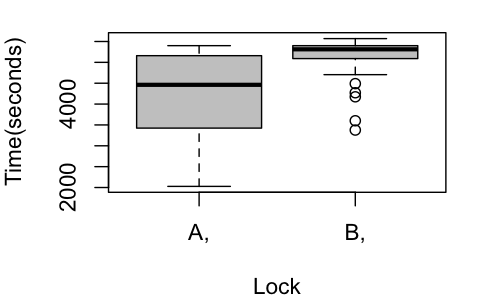
\includegraphics[height=4.5cm]{img/u1.png}
\caption{First experiment box-plot graphic.}\label{fig:boxplot1}
\end{figure}

\begin{table}
\centering
\begin{tabular}{|l|l|l|}
\hline
 & Time Spent (seconds)\\
\hline
LockA & 4227.800 \\
LockB & 5086.367 \\
\hline
\end{tabular}
\caption{First experiment's average time spent}\label{tab:mean1}
\end{table}

Then we run the Box-Cox transformation - a power transformation - to reduce anomalies such as non-additivity and non-normality.
First we verify if the transformation is needed, obtaining the curve in the left of Figure~\ref{fig:transf1}.
Since the value of {\tt lambda} at the maximum point in the curve is not approximately 1, we should apply it.
In order to apply the transformation, $Y_{lijk}$ should be powered to that $\lambda$ on our regression model.
Now, using the transformed model, we obtain the curve shown in the right of Figure~\ref{fig:transf1}.

\begin{figure}
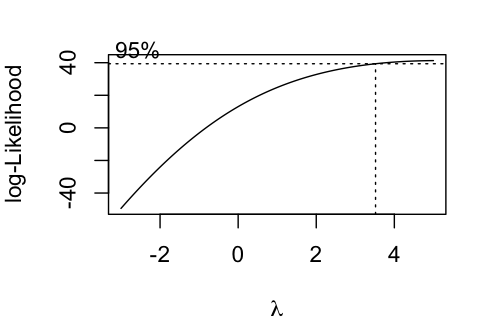
\includegraphics[height=4.5cm, width=6cm]{img/u2.png}
\hfill
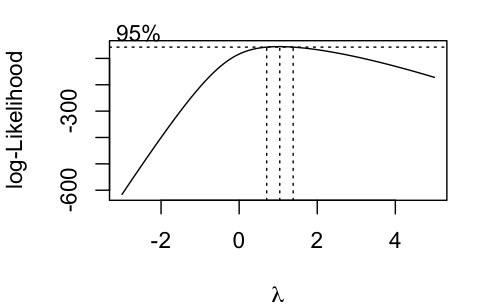
\includegraphics[height=4.3cm, width=6cm]{img/u2boxcox.png}
\caption{First experiment: before and after box-cox transformation ($\lambda = 5$).}\label{fig:transf1}
\end{figure}

In the next step we ran Tukey Test of Additivity to check whether effect model was additive.
Interaction between factors displayed on rows and columns of each latin square won't affect significantly the response only when the model is additive~\cite{box},
so we must verify it (Figure~\ref{tab:tukey}).

\begin{figure}
\centering
\begin{tabular}{ll}
$H_{0}$ & : The model is additive \\
$H_{1}$ & : $H_{0}$ is $false$ \\
\end{tabular}
\caption{Tukey Test of Additivity hypothesis}\label{tab:tukey}
\end{figure}

When the test was executed, we obtained p-value of 0.514, which means we cannot reject $H_{0}$.
Consequently the model was considered to be additive.

Finally, we ran the ANOVA (ANalysis Of VAriance) test which compares the effect of treatments on the response variable,
providing an approximated p-value for every associated factor (see Table~\ref{tab:anova1}).
When a variable has p-value $< 0.05$, it means that factor was statistically significant to the response.
It shows that {\bf lock factor was the most significant to the response}, allowing us to reject our null hypothesis defined in Equation 10.

\begin{table}
\begin{center}
\caption{Undergraduate students experiment ANOVA results.}\label{tab:anova1}
\begin{tabular}{|l|l|l|l|l|ll|}
\hline
                & Df &    Sum Sq  &  Mean Sq   & F value & \emph{p-value} &     \\  
Replica         & 14 & 3.8633e+37 & 2.7595e+36 & 1.6553  & 0.1784197 &     \\   
Program         & 1  & 4.1460e+36 & 4.1460e+36 & 2.4869  & 0.1371197 &     \\   
Lock            & 1  & 3.9489e+37 & 3.9489e+37 & 23.6873 & 0.0002492 & *** \\
Replica:Student & 15 & 4.1013e+37 & 2.7342e+36 & 1.6401  & 0.1808595 &     \\  
Replica:Lock    & 14 & 2.4033e+37 & 1.7166e+36 & 1.0297  & 0.4785520 &     \\  
Residuals       & 14 & 2.3340e+37 & 1.6671e+36 &         &           &     \\
\hline
\end{tabular}
\end{center}
\end{table}

Now we will show the results collected by the second experiment with graduate students. They were exposed to the same set of problems in a different day, but as explained before, they only had a time limit of 1 hour per question.

When we analyze the box-plot for the second group (Image~\ref{fig:boxplot2}) and their average time spent (Table~\ref{tab:mean2}), we can see there was a clear improvement on the time for students using \emph{LockA}.

\begin{figure}
\centering
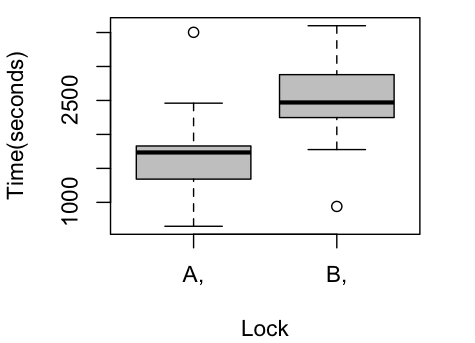
\includegraphics[height=4.5cm]{img/g1.png}
\caption{Second experiment box-plot graphic.}\label{fig:boxplot2}
\end{figure}

\begin{table}
\centering
\begin{tabular}{|l|l|l|}
\hline
 & Time Spent (seconds)\\
\hline
LockA & 1737.714 \\
LockB & 2507.714 \\
\hline
\end{tabular}
\caption{Second experiment's average time spent}\label{tab:mean2}
\end{table}

Moving foward with the analysis, we check if a box-cox transformation is needed. Since the value is not approximately 1, we apply the power transformation the same way we did with the first experiment, but with the corresponding lambda value.

\begin{figure}
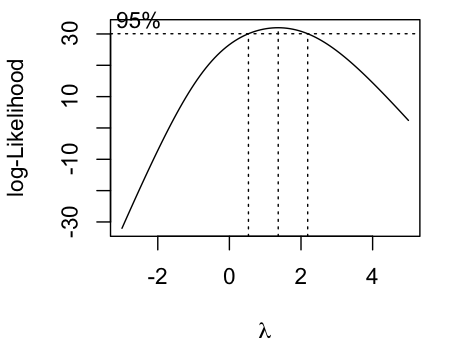
\includegraphics[height=4.5cm]{img/g2.png}
\hfill
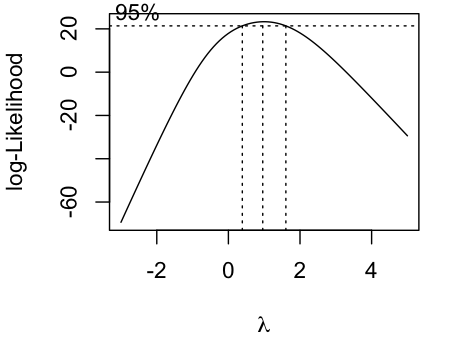
\includegraphics[height=4.4cm]{img/g2boxcox.png}
\caption{Before and after box-cox transformation ($\lambda = 1.3636$).}\label{fig:transf2}
\end{figure}

Finally, running ANOVA, we can see that the type of lock was the most significant factor for the response time, as shown in Table~\ref{tab:anova2}. Again, we can reject the null hypothesis.

\begin{table}
\begin{center}
\caption{Graduate students ANOVA results.}\label{tab:anova2}
\begin{tabular}{|l|l|l|l|l|ll|}
\hline
                 & Df &    Sum Sq &   Mean Sq  & F value &   Pr(>F) & \\   
\hline
replica          & 6 & 2576883250 &  429480542 & 14.1891 & 0.0025793 & **  \\
program          & 1 &    6875586 &    6875586 &  0.2272 & 0.6505035 &     \\
lock             & 1 & 1958179433 & 1958179433 & 64.6938 & 0.0001975 & *** \\
replica:student  & 7 & 2328154077 &  332593440 & 10.9881 & 0.0047601 & **  \\
replica:lock     & 6 &  823830276 &  137305046 &  4.5362 & 0.0441188 & *   \\
Residuals        & 6 &  181610625 &   30268438 &         &           &     \\
\hline
\end{tabular}
\end{center}
\end{table}

\subsubsection{Accuracy Analysis.}

We used the number of correct answers using each lock to measure accuracy, so we defined the following hypothesis to answer {\bf RQ2}. 

\begin{equation}
  H_{0} : \mu_{CorrectAnswersLockA} \leq \mu_{CorrectAnswersLockB}
\end{equation}
\begin{equation}
  H_{1} : \mu_{CorrectAnswersLockA} > \mu_{CorrectAnswersLockB}
\end{equation}

Once we collected all answers, we manually evaluated each one of them according to the criterias established previously, where each criteria had an associated value between 0 and 1. Then we've ran a script that evaluates the equation we defined before to classify whether an answer was correct or not. Grouping the results in tables, we have Table~\ref{tab:acc1} and Table~\ref{tab:acc2}.

\begin{table}
\begin{center}
\caption{Undergraduate students answers accuracy}\label{tab:acc1}
\begin{tabular}{|l|l|l|}
\hline
 & Correct & Incorrect\\
\hline
LockA & 29 & 2\\
LockB & 16 & 15\\
\hline
\end{tabular}
\end{center}
\end{table}

\begin{table}
\begin{center}
\caption{Graduate students answers accuracy}\label{tab:acc2}
\begin{tabular}{|l|l|l|}
\hline
 & Correct & Incorrect\\
\hline
LockA & 13 & 1\\
LockB & 10 & 4\\
\hline
\end{tabular}
\end{center}
\end{table}

Applying Fisher's exact test we can see that undergraduate students results presented a two-tailed P value equals 0.0004: the association between rows (groups) and columns (outcomes) is considered to be extremely statistically significant; consequently, there is clear evidence of improvement on accuracy (see Table~\ref{tab:acc1}).

Meanwhile graduate students results presented a two-tailed P value equals 0.3259, which does not represent a statistically significant evidence of improvement in accuracy (see Table~\ref{tab:acc2}).

% TODO: add script and the data used (anonymized) to appendices or put on github and link %

\subsection{Discussion}

% TODO: review this section, it was written based on older results %

We can see in our results that both groups of students have improved their time to solve the problem when they had the lock with deadlock exception. Also, on the first group, we have found statistically significant evidence that it improved answers accuracy, but not for the second group.

We cannot draw conclusions regarding the improved accuracy on the second group, but we can bring up some relevant aspects we've observed and make a few hypothesis. Some students in the second group were greatly experienced on concurrent programming and they knew how to efficiently find a deadlock using the tools available in Eclipse. Thus, they have finished the exercise really quickly for both problems, knowing exactly which points in the code were involved in the deadlock. So we can see that deadlock exceptions are more helpful for unexperienced programmers in general, and it's possible that even if we had a bigger sample for the second group, we would still not see a significant difference that would indicate deadlock exceptions improved their accuracy.

However, we believe that the benefits of deadlock exceptions are beyond helping unexperienced programmers to find deadlocks more precisely. Experienced programmers would still benefit in many cases where the deadlock is not as obvious as in the exercise we've presented. For example, in a more realistic situation, a deadlock can happen in a background thread that doesn't really affect the program execution overall but make the execution lacking some expected behavior. Furthermore, in non-interactive systems where they are only running in background, is nearly impossible to know when there's a problem unless this software is monitored constantly which is very time consuming or the system produces output constantly that is affected by a potential deadlock. If we have a deadlock exception, we can either prepare and handle this exception on the code level, or just have this signal from output that would help developers to fix it later.

\subsection{Threats To Internal Validity}

In this experiment, we've collected evidence on how the presence of deadlock exception affects student ability to identify deadlocks accurately. However, we must raise a few considerations regarding the validity of our results.

\subsubsection{Time Measurement.}

Since we wanted to run the experiment in a homogenous environment, we've decided to run it in a laboratory in Federal University of Pernambuco, and we've provided links to download the exercise and a few instructions explaining how to deploy it. We wanted to make it as easy as possible and before we've started the test, we gave a small presentation reproducing step by step the instructions that would be described on each exercise, so everyone could follow up and make the setup at the same time. Once everyone was done, we've started to count the time and allowed them to run the programs and start debugging. However, this procedure was not enough: there was a few students (approximately 3 in total) who did the setup differently and could not execute the program; therefore, they've lost a few minutes until we've fixed that for them. Since they've lost only a few minutes, we have still counted them as part of the experiment and did not discount the time.

Furthermore, some students arrived at the test more than 10 minutes late. We've allowed them to join, but some of the remaining computers in the laboratory had issues like they were not logging in or the mouse was not working. We've lost a few minutes to make them work or find a new computer and once each of them did the setup, we've started to count their time individually.

Whenever a student finished a given question, if the time was below the time limit they had available, we have marked the current timestamp on each student's name in the whiteboard. Each entry inserted was already sorted by time, so we easily tracked whether each student was close to the second question's time limit. It would have been better to do this automatically rather than doing manually, so we could potentially reduce overhead of these timestamp operations and increase their precision.

Also, we believe that our imposed time limit have limited more drastically the time ranges on the first group because they spent more time on each question. Also the fact it was an exam for them may have delayed the time to answer because they were more careful. We have observed during the experiment that many students wrote their answers but they were reluctant to ask for the next question because they still have plenty of time left and they wanted to make sure it was correct. We did not observe such behavior with the second group of students and we believe it is because they did not have the same pressure to deliver correct results as the first group had.

\subsubsection{Exercises.}

We understand that the two questions we've used to evaluate the students are far easier than what most software engineers have to deal with in the real world. However we could not use any real world issue because it would easily take the time limit of the experiement for each bug.

On the other hand, we've created two questions based on real world bugs that we have found while searching for deadlock bugs in open source repositories. Each question had a particular level of granularity, where one should be easier to find a bug because of the less amount of code to examine and another that should be more difficult because of the reasonable amount of different files to look at.

Some researchers actually believe that empiric evaluations should not be limited to real projects. Buse claims there are benefits of using non-real artifacts \cite{buse} because it's easier for researchers to translate research questions into successful experiments as it allows a greater control over confouding factors. Otherwise, it would be necessary to turn all participants familiar with the codebase of a real and complex system before even starting the experiment. 

\subsection{Threats to External Validity}

Let's consider a few conditions that might limit the generalization power of our findings in this experiment.

\subsubsection{Students.}

Each student which participated in this experiment had a different background. What we did to minimize the differences was to select groups where students had at least basic experience in concurrent programming and they should be familiarized with the types of bugs such codes can have: the first group of students with undergraduate students attended the class Paradigms of Computaional Languages where deadlocks are covered in classes and exercises; the second group with graduate students attended the class Parallel Programming which covered concurrent programming in low level detail in classes and exercises, including deadlock detection.

Some studies have already addressed the problem of drawing conclusions made with students but some suggest that using students as subjects is as good as using industry professionals \cite{staron}. Runes ran an experiment which shows that there's not much significant differences between undergraduate, graduate and industry professionals, with the exception that undergraduate students often take more time to complete the tasks \cite{runes}.

\subsection{Performance Overhead}\label{sec:perf}

We conducted a preliminary set of experiments to analyze the overhead of our approach.
We compared the our implementation of ReentrantLock with deadlock exceptions, the original ReentrantLock and Eclipse's {\tt OrderedLock}~\cite{orderedlock} implementation in a synthetic benchmark.

OrderedLock is a deadlock-safe implementation of a lock which relies on Eclipse's code architecture.
It is similar our approach in the sense that it attempts to detect deadlocks at runtime. However, it aims to be general, detecting $N$-thread deadlocks without much concern for performance: when a deadlock happens, it releases all locks by a given thread and suspends it, allowing other threads to proceed;
later, the suspended thread will acquire such locks again.
Since it allows threads to temporarily give up all its owned locks, it loses the property of guaranteeing exclusive access policy in \emph{critical zones} that all locks should provide.
In order to use it in our evaluation, as it deeply relies on Eclipse's code architecture to function, we had to perform some small code changes, removing only Eclipse-specific bits that did not affect the core functionality of OrderedLock.
The source code for these lock implementations is available elsewhere~\cite{repo}.

We developed a synthetic benchmark that creates \emph{N} threads that perform additions to ten integer counters where each increment in a counter is protected by explicit locks. Each thread would have to increment its corresponding counter 1000 times before finishing its execution and the counters were evenly distributed across the threads. Therefore, each counter will have exactly \emph{(N / 10)} threads doing increments on it and higher values of \emph{N} result in higher contention, that is, more threads will compete against each other for a particular counter. In this preliminary evaluation, we have conducted measurements for values of $N$ equal to 10, 50, 100, and 200. Since each thread in the benchmark never acquires more than one lock at the same time, deadlocks cannot occur. We emphasize that this setup is very conservative, since every operation that each thread performs requires locking. Thus, the obtained overhead will be a worst-case estimate and thus much higher than one would encounter in a real-world application~\cite{lozi}. The measurements were made on an Intel CoreTM i7 3632QM Processor (6Mb Cache, 2.2GHz) running Ubuntu 12.04.4 LTS and each cell in Table~\ref{tab:overhead} is the average of 50 executions (preceded by 20 executions that served as a warm-up).

\begin{table}
\begin{center}
\caption{Benchmark time measurements (in seconds)}\label{tab:overhead}
\begin{tabular}{|l|l|l|l|}
\hline
\# Threads & ReentrantLock & ReentrantLock Modified & OrderedLock \\
\hline
10 & 0.084184 & 0.105729 & 0.159503\\
50 & 0.089094 & 0.136507 & 1.094718\\
100 & 0.090978 & 0.159541 & 3.395974\\
200 & 0.131739 & 0.194075 & 11.258714\\
\hline
\end{tabular}
\end{center}
\end{table}

The difference of results between our implementation and the original ReentrantLock gives a range of increased time from about 50\% to 90\%. Meanwhile, OrderedLock performed a lot worse, reaching a 8446.3\% increase in time for the worst case. To get a rough estimate of the impact that this overhead would have on actual application execution time, we analyzed the results obtained by Lozi et al.~\cite{lozi}. The authors profiled 19 real-world applications and small benchmarks in order to measure the time these systems spend on their critical sections. Worst-case results ranged between 0.3\% and 92.7\%. If we consider the average time spent on the critical sections of 12 of these systems, the impact of our approach on the overall execution time would be \textbf{less than 6\% in the worst case}. The remaining cases are extreme, in the sense that these systems spend more time in their critical sections than out of them~\cite{lozi}. 




\section{Foundation}

In this section, we will cover the basic concepts and previous studies related to deadlock detection. We're going to to start by covering topics such as static analysis, dynamic analysis and hibrid analysis, citing previous studies that contributed into those categories.

\subsection{Static Analysis}

Static analysis techniques verify source code from a program and try to identify potential problems present in the code without even executing it.
For deadlock detection, they generally attempt to detect cyclic relationships of resource acquisition between threads where each cycle represents a possible deadlock.
Many static analysis approaches were proposed over the past decade \cite{dawson}\cite{chand}\cite{vivek}\cite{praun}\cite{cormac}\cite{williams}
but in general they suffer of signficant amount of false positives being reported as there may exist deadlock cycles that are just impossible to happen during execution.
Also, some deadlocks cannot be detected when the language is weakly typed, such as C/C++.

Recently, Marino et al. \cite{marino} proposed a static analysis technique to detect potential deadlocks in programs that
used an extension of Java called AJ that implements atomic sets for class fields as an abstraction of locks to prevent data races
and atomicity violations by construction. Its declarative nature allows the algorithm to infer which locks each thread may acquire and
compute a partial order for those atomic sets which would also be consistent with lock acquisition order.
If such order was detected, the program was guaranteed to be deadlock-free, otherwise possible deadlock would be reported.
It was implemented as extension of their existing AJ-to-Java compiler and synchronization annotations were given as special Java comments in the code.
These comments would be parsed and given to the type checker to execute the deadlock analysis. AJ source code would be translated to Java and written into a separated project
with the transformed code which would later be compiled into bytecode and executed by JVM. A limitation of this approach is that AJ is a research language
and does not have real users, thus obtaining suitable subject programs to do any evaluation was difficult, and their chosen projects to evaluate might not
represent concurrent programming styles that occur in practice, but at least for most of the subject programs analysed, deadlock-freedom could be demonstrated
without any programmer intervention.

\subsection{Dynamic Analysis}

Dynamic analysis finds potential deadlock cycles from an execution trace of a program which makes them often more scalable and precise than static analysis.
However, due to the sizes of large-scale programs, the probability that a given run will show a thread acquiring a lock at the right time to trigger a deadlock for
each potential deadlock present in the code is very low, which poses a challenge for dynamic deadlock detection tools. Thus if a given run does not identify potential
deadlocks, it does not mean the program is free from deadlocks either. Another disadvantage of dynamic analysis is that they often incur runtime overhead and most techniques
can't be applied in real-world applications for lack of scalability.

Zuo et al. \cite{mcsdk} present a dynamic deadlock detection tool called MulticoreSDK which consists of two phases.
In the first phase, the algorithm works offline by examining a single execution trace obtained after an instrumented program finishes its execution,
creating a lightweight lock graph based on program locations of lock events and identifying locks that may be deadlock-related in this graph by checking cycles on it.
Second phase consists of examining the execution trace and constructing a filtered lock graph based on the lock id of each lock event, analysing only deadlock-related locks
found in the first phase. Each cycle found in this final graph is reported as potential deadlock in the program.
It works for java programs and its instrumentation is done by deploying a bytecode instrumentation technique \cite{tanter} to insert extra bytecode
around instructions such as \emph{monitorenter} and \emph{monitorexit} which would record the thread and the id of lock objects, also around methods lock and unlock of
\emph{Lock} interface in java.util.concurrent package and enter/exit of synchronized methods.
Although the algorithm requires to pass over the program trace twice, most of its performance overhead is consumed in the deadlock analysis itself.
When compared with a traditional approach \cite{contest}, MulticoreSDK has a very small performance gain in analysis time on small applications while memory consumption
was reduced by about half; meanwhile, for large applications, about 33\% performance gain was reached, consuming about 10 times less memory.

Cai et al. \cite{magicfuzzer} present a dynamic analysis technique known as MagicFuzzer which consists of three phases.
First phase consists of critical events such as a thread creation or lock acquisition and release being monitored in a running program to generate
a log of series of lock dependencies which can be viewed as a lock dependency relationship.
On the second phase, the algorithm classifies such relations in a cyclic-set which contains all the locks that may occur in any
potential deadlock cycles found in a given execution.
Then it constructs a set of thread-specific lock-dependency relations based on the locks inside that cyclic-set which is finally tranversed to find potential deadlock cycles.
On the third phase, all deadlock cycles found in second phase are used as input to the program execution,
and it is actively re-executed to observe if any further execution will trigger any of those
potential deadlock cycles in the input, reporting the deadlocks whenever they occur, until all deadlocks are found or the limit of times to re-execute is reached.
One of its key differences is the presence of an active random scheduler to check against a set of deadlock cycles
which is said to improve the likehood that a match between a cycle and an execution will be found, but its proof is left open to future work.
It was implemented using a dynamic instrumentation analysis tool known as Pin 2.9 \cite{pin} which only works for C/C++ programs that use Pthreads libraries on a Linux System.
It was tested on large-scale C/C++ programs such as \emph{MySQL} \cite{mysql}, \emph{Firefox} \cite{firefox} and \emph{Chromium} \cite{chromium},
and for some of them, the test would simple start the program and then close it when the interface appeared, while other programs used test cases adopted
from bug reports in their own repositories. After evaluating the results of tests, it was concluded that it could run efficiently with low memory consumption
if compared to similar techniques, like MulticoreSDK \cite{mcsdk}.

Pyla et al. \cite{sammati} presents Sammati as a dynamic analysis tool which is capable of detecting deadlocks automatically and
recovering for any threaded application that use the pthreads interface without any code changes, transparently detecting and resolving deadlocks.
It is implemented as a library that overloads the standard pthreads interface and turn locks into a deadlock-free operation.
By associating memory accesses with locks and specifying ownership of memory updates within a critical section to a set of locks,
it makes memory updates to be only visible outside of the critical section when all parent locks are released.
When a deadlock is detected, one of the threads involved in the deadlock is
chosen as a victim and rolled back to the point of acquisition of the offending lock, discarding memory updates done.
This way it would be safe to restart the code that runs into that critical section again because the memory updates never
were made visible outside of the critical section. Differently from transactional memory systems,
its performance impact is minimized because its runtime privatizes memory at page granularity instead of instrumenting
individual load/store operations. Containment for threaded codes was implemented with a technique described in \cite{berger}:
if each thread had its own virtual address space, such as most recent UNIX operating systems,
privatization can be implemented efficiently in a runtime environment where threads are converted to \emph{cords} which is a single threaded process.
In this algorithm, threads are converted to cords transparently, and since all cords share a global address space, the deadlock detection algorithm
has access to the holding and waiting sets of each cord and the deadlock detection can be performed at the time a lock is acquired.
Its detection algorithm uses a global hash table that associates locks being held with its owning cord, another hash table to associate a cord with a lock it is waiting on and a
queue per cord of locks acquired. Its deadlock detection complexity is linear and has upper bound of $\mathcal{O}$(n) where n is the number of threads.
However, rollback of acquired locks and all its related memory changes adds a high runtime overhead, given the high costs related to its address space protection
and privatization logic. Also, there are some limitations in what kind of memory can be recovered in a rollback, like
non-idompotent actions (i.e. I/O, semaphores, condition signals, etc.) and shared libraries state \cite{pyla}.
Part of these limitations were addressed with Serenity \emph{serenity}, like serializing some disk I/O operations within critical sessions,
and it will be discussed further in the next section.

Qin et al. \cite{rx} proposes a dynamic approach called Rx that rolls back a server application once a bug occurs to a checkpoint,
trying to modify the server environment on its re-execution. In that study, bugs are treated as "allergies" and different program executions
could either have the "allergen" or not. In the context of concurrency bugs such as deadlocks, as timing is essential for deadlocks to manifest,
a retry of the server request that caused a deadlock could be enough to get rid of the deadlock.
It works by dynamically changing the execution environment based on the failure symptoms, and then
executing again the same code region that contained the bug, but now in the new environment.
If the re-execution successfully pass through the problematic period,
all environment changes are disabled thus time and space overheads are avoided.
Intercept of memory-related library calls (i.e. \emph{malloc()}, \emph{realloc()}, etc.) was implemented on a memory wrapper
in order to provide environmental changes. During normal execution, it will simply invoke the corresponding
standard memory management library calls, which incurs little overhead. Then at re-execution phase (called \emph{recovery} mode), the memory wrapper would activate
a memory-related environmental change instructed by the control unit. Its evaluations shows that it recovered from software failure in about 0.16 seconds which was
significantly better compared to what was done before (web application restart).

\subsection{Hybrid Analysis}

It is also possible to mix both static analysis and dynamic analysis in an hybrid analysis to take advantage of both types and boost performance during runtime.
Some techniques deploy static analysis to infer deadlock types and dynamic analysis for the parts of the program that could not be analysed in the first part,
reducing the overhead caused by dynamic analysis drastically.

Grechanik et al. \cite{grechanik} proposes REDACT that would statically detect all hold-and-wait cycles among resources in SQL statements
and prevent database deadlocks dynamically by running a supervisory program to intercept transactions sent by applications to databases.
Once a potential deadlock is detected, the conflicting transaction is delayed which results on breaking the deadlock cycle.
As database deadlocks may degrade performance significantly, it tries to prevent them of happening.
An static analysis is executed at compile time and later used at runtime, allowing its deadlock detection algorithm to just make simple lookup
in the hold-and-wait cycles already detected in compile time, improving deadlock detection performance compared to similar techniques.
In the first step, some manual-effort is required on every application to build all database transactions used in the application,
which allows static analysis phase to begin. Its results are parsed and used to generate hold-and-wait cycles necessary by the runtime detection algorithm.
The dynamic phase is responsible to prevent database deadlocks automatically. It adds interceptors in the application with callbacks associated with particular events and
instead of sending SQL statements from application to the database, they divert the statements to the supervisory controller whose goal is to quickly analyse if
hold-and-wait cycles are present in the SQL statements that are in the execution queue. If no hold-and-wait cycle is present, then it forwards these statements to the
database for execution normally. Otherwise, it holds back one SQL statement while allowing others to proceed,
and once these statements are executed and results are sent back to applications,
the held back statement is finally executed by the database.
Some of its limitations include that not all hold-and-wait cycles detected in the static analysis will actually lead to database deadlocks, so false positives are still possible.
Databases are highly optimized against deadlocks, so even though some obvious deadlock should happen in theory, in practice they would be prevented by the database itself, but
this approach will handle such cases as if a deadlock would happen anyway and consequently imposes an overhead in addition to some reduction in the level of parallelism in applications.
Also, when the static analysis produces too many false positives of hold-and-wait cycles, there is a significant performance overhead overall.

Pyla et al. presents Serenity \cite{serenity} as a sucessor of Sammati \cite{sammati} to handle some previous limitations by mixing some runtime analysis with
its previous runtime approach, so they share many similarities.
Program analysis and compile time instrumentation were used in Serenity to guide runtime and efficiently achieve memory isolation with
some static analysis techniques to infer the scope of a lock and using selective compile time instrumentation on those identified scopes.
In order to handle some previous I/O limitations, Serenity serializes disk I/O operations performed within critical sections and marks
threads that performed some of these operations.
When a deadlock is detected, differently from \cite{sammati}, it will choose as victim a thread that did not perform I/O inside any lock context.
It also tracks all disk I/O primitives (i.e. read, write, etc.) and all thread creation/termination primitives (i.e. fork, clone,
etc.) as I/O operations to verify whether such operations were performed within a lock context.
The new approach also has its own limitations, as it cannot recover from certain deadlocks such as arbitrary I/O within the context of a restartable critical section \cite{pyla}.
It also requires some programmer input if lock/unlock operations are encapsulated in functions/classes,
so they should be explicitly identified by the developer before running its compile time analysis.
Furthermore, recompiliation is now necessary for application and all its external dependencies (i.e. shared libraries) in order to also instrument them.

\subsection{Deadlocks as Exceptions}

Deadlock detection or recovery algorithms are not always as efficient or reliable as they should be, as we've seen in the previous sections.
Some techniques generates false positives as deadlocks candidates, other techniques imposes high runtime overhead. Some also offer recovery from
deadlocks automatically, but they don't work if certain operations happen inside critical sections. Finally, some techniques are too specific
to the type of application (such as webservers or databases) and they are not easily translated into other application types efficiently.

Building deadlock-free programs is an old challenge.
Concurrent Pascal \cite{hansen} was presented in 1975 as a language with a compile-time deadlock detection built-in. It had several
limitations such as fixed amount of processes and recursive functions not allowed, but then it could process a partial ordering
of process interactions and prove certain system properties such as absence of deadlocks during compilation.

In modern languages and databases systems, deadlocks are nothing but bugs, and they have exceptions in few special cases.
Database deadlocks are typically detected within database engines at runtime \cite{grechanik} raising deadlock exceptions and rolling back transactions
involved in the circular wait. Haskell programming language throws deadlock exceptions when garbage collector detects a thread as unreachable\footnote{http://goo.gl/v09kqn}
and no other thread can wake it up. Another programming language, Go, throws deadlock exception when all \emph{goroutines} are blocked waiting on their message channel\footnote{http://guzalexander.com/2013/12/06/golang-channels-tutorial.html}.

We believe the presence of deadlock exceptions in programming languages are very useful specially when it's guaranteed to be fired and programmers can rely upon it.
The main advantage is that they inform there's something unexpectedly wrong in the code which allows programmers to identify the problem easier and potentially fix it faster.
Furthermore if the exception is guaranteed to be fired then programmers can have specialized code to run when it happens.

For instance, a deadlock exception could be handled in the code to trigger some deadlock recovery mechanism specialized for that case, if it is indeed necessary.
This approach has an advantage on its own because it does not rely on any auto-recovery mechanism as seen in some previous deadlock detection algorithms,
because they were in general very inneficient. Thus, automatically recovering from deadlocks could potentially cover real bugs that needs to be fixed immediately
and also turn application's performance a lot worse in exchange.

In non-interactive systems, there's a huge benefit of having deadlock exceptions in the programming language.
Currently, it is very difficult to find a deadlock when it happens but it's a lot harder when the system is not monitored constantly, as non-interactive systems usually are.
In Pie at all's paper \cite{ian}, it is discussed how difficult it was to identify one of the concurrency bugs which was just a classical deadlock (two threads circularly waiting each other). However, the deadlock did not leave the application completely stuck, but instead an intended behaviour in a specific case did not happen because of this hidden deadlock
which made the problem very hard to debug and be identified.

We want to solve this problem by extending programming languages to support deadlock exceptions. We believe they can help developers to find and fix their mistakes
in the code when they have such exception. However we want to solve this problem efficiently too, then we decided to focus on the most common type of deadlock:
two threads and two locks, waiting for each other. In this study, we've extended \emph{Lock} interface in java.util.concurrent package in Java OpenJDK to support
a runtime exception called \emph{DeadlockException}. It was later tested with students to measure how its presence could improve their ability to accurately identify issues in the code.
We will present the implementation of this deadlock algorithm and its evaluation with students in the following chapters.

%\section{Future Work}

As a proposal for future work, runtime exception should also be added to synchronized blocks in Java while trying to maintain runtime overhead as low as possible.
That way, it would allow easier integration with existing software as many programmers prefer to use synchronized blocks instead of explicit locks,
and also it would be possible to do a better performance impact analysis using real world applications instead of synthetic benchmarks.

Another idea is to push these changes to Java's \emph{ReentrantLock} forward and add native support for DeadlockException in Java JDK,
but some optimization in our algorithm might be needed as well to reduce even more the runtime overhead as we've seen in our benchmark in this work.

\section{Conclusion}

In this work, we've initially discussed how challenging it is to handle deadlocks and resolve them in real world software, and present many previous approaches that
have tried to identify or solve deadlocks with either static analysis, dynamic analysis or a mix of the two approaches.

Given that it's very costly to detect deadlocks in its general form, we've investigated which kind of deadlock is the most popular by looking at actual bug reports
in relevant open source projects and classifying each deadlock manually. We've confirmed a previous study claim that classic deadlocks between two threads and two resources
are the most frequent case of deadlock. This claim allowed us to focus on this specific case instead and minimally modify Java's \emph{ReentrantLock} to provide a lightweight
version of a lock that detects this kind of deadlock in runtime.

However, differently from previous approaches, we provided a runtime exception which should be raised on both threads involved in a classic deadlock
when our Java's \emph{ReentrantLock} implementation is used, as we believe that developers would find bugs faster if deadlocks were just exceptions.

Our usability evaluation with students shows that the presence of deadlock exception indeed reduce the amount of time spent to identify a bug in a code they were not familiar with. It also shows that less experienced students could identify the source of the deadlock correctly more easily, and we believe these results are very promising.

Finally, we summarize our main contributions in this work as follows:
\begin{enumerate}
\item Found evidence that classic deadlocks are the most popular type of deadlock (92.07\% of all resource deadlocks we've identified);
\item Provided an implementation of reentrant lock that detects classic deadlocks and throw runtime exception on both threads, preceded by a sketch of a proof that shows why this detection algorithm works;
\item Found evidence that deadlock exception reduces time to identify problems and can also improve the ability to identify deadlocks correctly for less experienced developers.
\end{enumerate}

\chapter{Bibliography}

\begin{thebibliography}{4}

\bibitem{lu} Lu, Shan, et al: Learning from mistakes: a comprehensive study on real world concurrency bug characteristics.
ACM Sigplan Notices. Vol. 43. No. 3. ACM, 2008.

\bibitem{singhal} Singhal, Mukesh. Deadlock detection in distributed systems.
Computer 22.11 (1989): 37-48.

\bibitem{knapp} Knapp, Edgar: Deadlock detection in distributed databases.
ACM Computing Surveys (CSUR) 19.4 (1987): 303-328.

\bibitem{marino} Marino, Daniel, et al: Detecting deadlock in programs with data-centric synchronization.
Software Engineering (ICSE), 2013 35th International Conference on. IEEE, 2013.

\bibitem{dolby} Dolby, Julian, et al: A data-centric approach to synchronization.
ACM Transactions on Programming Languages and Systems (TOPLAS) 34.1 (2012): 4.

\bibitem{mcsdk} Da Luo, Zhi, Raja Das, and Yao Qi: Multicore sdk: a practical and efficient deadlock detector for real-world applications.
Software Testing, Verification and Validation (ICST), 2011 IEEE Fourth International Conference on. IEEE, 2011.

\bibitem{tanter} Tanter, Éric, et al: Altering Java semantics via bytecode manipulation.
Generative Programming and Component Engineering. Springer Berlin Heidelberg, 2002.

\bibitem{contest} ConcurrentTesting - Advanced Testing for Multi-Threaded Java Applications, \url{https://www.research.ibm.com/haifa/projects/verification/contest/}

\bibitem{magicfuzzer} Cai, Yan, and W. K. Chan: MagicFuzzer: scalable deadlock detection for large-scale applications.
Proceedings of the 2012 International Conference on Software Engineering. IEEE Press, 2012.

\bibitem{pin} Luk, Chi-Keung, et al. Pin: building customized program analysis tools with dynamic instrumentation.
ACM Sigplan Notices 40.6 (2005): 190-200.

\bibitem{mysql} MySQL, available at: \url{http://www.mysql.com}

\bibitem{firefox} Firefox, available at \url{http://www.mozilla.org/firefox}

\bibitem{chromium} Chromium, available at \url{http://code.google.com/chromium}

\bibitem{sammati} Pyla, Hari K., and Srinidhi Varadarajan: Avoiding deadlock avoidance.
Proceedings of the 19th international conference on Parallel architectures and compilation techniques. ACM, 2010.

\bibitem{rx} F. Qin, J. Tucek, Y. Zhou, and J. Sundaresan. Rx: Treating bugs as
allergiesa safe method to survive software failures. ACM Trans. Comput.
Syst., 25(3), Aug. 2007.

\bibitem{berger} Berger, Emery D., et al: Grace: Safe multithreaded programming for C/C++.
ACM Sigplan Notices. Vol. 44. No. 10. ACM, 2009.

\bibitem{splash} SPLASH-2. SPLASH-2 benchmark suite, available at \url{http://www.capsl.udel.edu/splash}

\bibitem{phoenix} Ranger, Colby, et al: Evaluating mapreduce for multi-core and multiprocessor systems.
High Performance Computer Architecture, 2007. HPCA 2007. IEEE 13th International Symposium on. IEEE, 2007.

\bibitem{grechanik} Grechanik, Mark, et al: Preventing database deadlocks in applications.
Proceedings of the 2013 9th Joint Meeting on Foundations of Software Engineering. ACM, 2013.

\bibitem{sanchez} Iván Sanchez. Latin Squares and Its Applications on Software Engineering. Master's thesis, Federal University of Pernambuco, Recife, Brazil, 2011.

\bibitem{paola} Paola Accioly. Comparing Different Testing Strategies for Software Product Lines. Master's thesis, Federal University of Pernambuco, Recife, Brazil, 2012.

\bibitem{buse} Raymond P. L. Buse, et al. Benefits and barriers of user evaluation in software engineering research. ACM SIGPLAN Notices, 46(10):643-656, October 2011.

\bibitem{runes} Per Runeson. Using students as experiement subjects - an analysis on graduate and freshmen student data. In Proceedings of the 7th International Conference on Empirical Assessment in Software Engineering. Keele University, UK, pages 95-102, 2003.

\bibitem{staron} Miroslaw Staron. Using students as subjects in experiments - A quantitative analysis of the influence of experimentation on students' learning process. In CSEE&T, apges 221-228. IEEE Computer Society, 2007.

\bibitem{box} G. E. P. Box, J. S. Hunter, and W. G. Hunter, Statistics for experimenters: design, innovation, and discovery. Wiley-Interscience, 2005.

\end{thebibliography}
%\begin{appendices}

\chapter{Sample Size Calculation In R}

\noindent
\begin{verbatim}
sample.size = function(c.lev, margin=.5,
                       c.interval=.05, population) {
  z.val = qnorm(.5+c.lev/200)
  ss = (z.val^2 * margin * (1-margin))/c.interval^2
  p.ss = round((ss/(1 + ((ss-1)/population))), digits=0)
  METHOD = paste("Recommended sample size for a population of ",
                 population, " at a ", c.lev,
                 "% confidence level", sep = "")
  structure(list(Population = population,
                 "Confidence level" = c.lev,
                 "Margin of error" = c.interval,
                 "Response distribution" = margin,
                 "Recommended sample size" = p.ss,
                 method = METHOD),
            class = "power.htest")
}

sample.size(95, 0.5, 0.05, 541)
\end{verbatim}

\chapter{Sample Analsysis in Python}

\noindent
\begin{verbatim}
import sys

f = open(sys.argv[1], "r")
headers = f.readline().split('\t')
lists = [ list() for i in xrange(4) ]

for line in f.readlines():
  data = line.split('\t')
  data = [ i.strip() for i in data ]
  unit = tuple((data[0], data[2], data[3], data[4], data[5], data[6]))
  group = ord(data[1])-ord('A')
  lists[group].append(unit)

total = 0
overall = len(lists[0]) + len(lists[3])
for u in lists[0]:
  if u[2] == u[3] and u[2] == '2':
    total += 1

print '== results =='
print 'found', str(total), 'deadlock bugs with 2 threads and 2 locks'
print 'found', str(overall), 'potential deadlock bugs'
print 'rate (worse case): ', str(float(total)/float(overall)*100), '%'
print 'rate (best case): ', str(float(total+len(lists[3]))/float(overall)*100), '%'
\end{verbatim}


\chapter{Fetch Bug Reports Data}

\noindent
\begin{verbatim}
import random
import sys
import datetime

import json
import urllib2
import os.path

f = open(sys.argv[1], "r")
headers = f.readline().split('\t')

path = './bugs/'
bugs = list()

for line in f.readlines():
  data = line.split('\t')
  data = [ i.strip() for i in data ]
  bugs.append(data[0])
  rep,bug_number = data[0].split('-')

  filepath = os.path.join(path, data[0] + '.xml')
  if os.path.exists(filepath):
    continue
  print 'fetching data for', data[0]
  url = ''
  if rep == 'ECLIPSE':
    url = ("https://bugs.eclipse.org/bugs/show_bug.cgi?" +
           "ctype=xml&id=" + bug_number)
  elif rep == 'JDK':
    url = ('https://bugs.openjdk.java.net/si/jira.issueviews:' +
           'issue-xml/' + data[0] + '/' + data[0] + '.xml')
  elif rep == 'LUCENE':
    url = ('https://issues.apache.org/jira/si/jira.issueviews:' +
           'issue-xml/' + data[0] + '/' + data[0] + '.xml')

  u = urllib2.urlopen(url)
  content = u.read()
  out = open(filepath, "wb")
  out.write(content)
  out.close()
  print 'done writing', filepath

def delta_hours(ts1,ts2):
  return round((ts2-ts1).total_seconds() / 60.0 / 60.0,2)

def import_timestamp_jira(str):
  s = str.split()
  s = ' '.join(s[1:5])
  return datetime.datetime.strptime(s, "%d %b %Y %H:%M:%S")

def import_timestamp_bugzilla(str):
  s = str.split()
  s = ' '.join(s[0:2])
  return datetime.datetime.strptime(s, "%Y-%m-%d %H:%M:%S")

def import_from_jira(bug):
  import xml.etree.ElementTree as ET
  tree = ET.parse('./bugs/'+bug+'.xml')
  root = tree.getroot()
  t = root.findall('channel')[0].findall('item')[0]
  created = t.findall('created')[0].text
  resolved = t.findall('resolved')[0].text
  ts1 = import_timestamp_jira(created)
  ts2 = import_timestamp_jira(resolved)
  c = t.findall('comments')
  comments = 0
  if len(c) > 0:
    comments = len(c[0].findall('comment'))
  return tuple((delta_hours(ts1,ts2),comments))

def import_from_bugzilla(bug):
  import xml.etree.ElementTree as ET
  tree = ET.parse('./bugs/'+bug+'.xml')
  root = tree.getroot()
  t = root.findall('bug')[0]
  created = t.findall('creation_ts')[0].text
  resolved = t.findall('delta_ts')[0].text
  ts1 = import_timestamp_bugzilla(created)
  ts2 = import_timestamp_bugzilla(resolved)
  comments = len(t.findall('long_desc'))
  return tuple((delta_hours(ts1,ts2), comments))

for bug in bugs:
  rep = bug.split('-')[0]
  r = tuple()
  if rep == 'ECLIPSE':
    r = import_from_bugzilla(bug)
  else:
    r = import_from_jira(bug)
  print str(r[0]) + '\t' + str(r[1])
\end{verbatim}

\chapter{Java ReentrantLock pseudocode}

\noindent
\begin{verbatim}
int state;
Thread owner;
Node head;
Node tail;

void lock() {
  if (!tryFastAcquire()) {
    slowAcquire();
  }
}

boolean tryFastAcquire() {
  if (!hasQueuedPredecessors() && COMPARE_AND_SET(state, 0, 1)) {
    setExclusiveOwner(currentThread());
    return true;
  }
  return false;	
}

// Returns true if current thread
// is the first in the queue or it's empty
boolean hasQueuedPredecessors();

void setExclusiveOwner(Thread thread) {
  owner = thread;
}

void slowAcquire() {
  // Creates and atomically enqueue node with current thread
  Node waiterNode = new Node();
  enq(waiterNode);

  // Try a few times to acquire the waiterNode and then park
  // until its predecessor wakes up this thread
  boolean failed = true;
  try {
    while (true) {
      if (waiterNode.pred == head && tryFastAcquire())) {
        setHead(waiterNode);
        failed = false;
        return;
      }
      if (shouldParkAfterFailedAcquire(waiterNode.pred, waiterNode))
        park();
    }
  } finally {
    if (failed)
      cancelAcquire(waiterNode);
  }
}

void release() {
  if (tryRelease()) {
    unparkSuccessor(head);
  }
}

boolean tryRelease(int releases) {
  if (currentThread() != owner)
    return false;
  setExclusiveOwner(null);
  setState(0);
  return true;
}

void park() {
  LockSupport.park(this);
}

// Wakes up successor of a given node in the waiting queue
// if necessary by using LockSupport.unpark on its successor.
void unparkSuccessor(Node);

// Cancel the waiting node and remove from waiting queue.
// If there's a successor parked, unpark it.
void cancelAcquire(Node);

// Atomically checks if the node is really the head
// of the queue and try fastPath codepath.
// On success, the node is dequeued from queue
bool tryFastAcquireIfHead(Node);

// Atomically enqueues node in the waiting queue. It repeately
// tries to COMPARE_AND_SET to update tail until succeeds.
// If head and tail are not initialized yet, there will be
// an extra COMPARE_AND_SET on head to a new Node and tail
// will be set as head.
void enq(Node);

// Make sure to park only when is guaranteed an unpark signal
// can be received. It decides based on specific protocol
// between predecessor of a given node and that node.
shouldParkAfterFailedAcquire(Node, Node);

// Returns Thread corresponding to the current thread
Thread currentThread();

// Disables the current thread for thread scheduling
// purposes unless the permit is available.
LockSupport.park();

// Makes available the permit for the given thread,
// if it was not already available.  If the thread
// was blocked on park then it will unblock.
LockSupport.unpark(Thread);
\end{verbatim}


\chapter{Instructions in R to evaluate time}
\noindent
\begin{verbatim}
exp1.dat = read.table(file="/Users/rafaelbrandao/r_input.dat", header = T)
attach(exp1.dat)

replica = factor(replica.)
student = factor(student.)
program = factor(program.)
lock = factor(lock.)

# Plot the box plot graphic using the response variable (time)
# associated with the locks with the following command

plot(time~lock,col="gray",xlab="Lock",ylab="Time(seconds)")

# We set the effect model that will serve as basis for posterior analysis.
# Notice that the factor student is associated with the factor replica since for
# each replica we used a different pair of students. We also included the factor
# lock associated with the replica.

anova.ql<-aov(time~replica+student:replica+program+lock+lock:replica)

library(MASS)
bc <- boxcox(anova.ql,lambda = seq(-3, 5, 1/10))
# If transformation is needed, we calculate lambda and use it:
# anova.ql<-aov(time**<lambda>~replica+student:replica+program+lock+lock:replica)
lambda <- bc$x[which.max(bc$y)]

TukeyNADD.QL.REP<-function(objeto1)
{
y1<-NULL
y2<-NULL
y1<- fitted(objeto1)
y2<- y1^2
objeto2<- aov(y2 ~ objeto1[13]$model[,2] +
objeto1[13]$model[,3]:objeto1[13]$model[,2]
+ objeto1[13]$model[,4]+ objeto1[13]$model[,5])
ynew <- resid(objeto1)
xnew <- resid(objeto2)
objeto3 <- lm(ynew ~ xnew)
M <- anova(objeto3)
MSN <- M[1,3]
MSErr <- M[2,2]/(objeto1[8]$df.residual-1)

F0 <- MSN/MSErr
p.val <- 1 - pf(F0, 1,objeto1[8]$df.residual-1)
p.val
}
TukeyNADD.QL.REP(anova.ql)

plot(anova.ql)
anova(anova.ql)
\end{verbatim}

\chapter{Undergraduate students's time results. Input used in R for analysis}
\noindent
\begin{verbatim}
replica, student, program, lock, time
1, 1, p1, A, 4996
1, 1, p2, B, 5367
1, 2, p1, B, 5070
1, 2, p2, A, 5260
2, 3, p1, A, 2700
2, 3, p2, B, 5306
2, 4, p1, B, 4490
2, 4, p2, A, 4017
3, 5, p1, A, 2340
3, 5, p2, B, 5290
3, 6, p1, B, 3377
3, 6, p2, A, 4473
4, 7, p1, A, 5400
4, 7, p2, B, 5360
4, 8, p1, B, 5400
4, 8, p2, A, 3641
5, 9, p1, A, 5400
5, 9, p2, B, 5400
5, 10, p1, B, 3600
5, 10, p2, A, 2406
6, 11, p1, A, 3290
6, 11, p2, B, 5370
6, 12, p1, B, 5400
6, 12, p2, A, 5320
7, 13, p1, A, 3424
7, 13, p2, B, 5356
7, 14, p1, B, 5400
7, 14, p2, A, 5160
8, 15, p1, A, 2593
8, 15, p2, B, 5279
8, 16, p1, B, 4705
8, 16, p2, A, 4535
9, 17, p1, A, 5160
9, 17, p2, B, 5430
9, 18, p1, B, 5250
9, 18, p2, A, 4246
10, 19, p1, A, 4967
10, 19, p2, B, 5413
10, 20, p1, B, 5400
10, 20, p2, A, 3804
11, 21, p1, A, 5280
11, 21, p2, B, 5160
11, 22, p1, B, 4174
11, 22, p2, A, 4886
12, 23, p1, A, 4271
12, 23, p2, B, 5569
12, 24, p1, B, 5400
12, 24, p2, A, 4788
13, 25, p1, A, 5400
13, 25, p2, B, 5239
13, 26, p1, B, 5310
13, 26, p2, A, 5390
14, 27, p1, A, 2027
14, 27, p2, B, 4271
14, 28, p1, B, 5090
14, 28, p2, A, 4450
15, 29, p1, A, 3000
15, 29, p2, B, 5315
15, 30, p1, B, 5400
15, 30, p2, A, 4210
\end{verbatim}

\chapter{Graduate students's time results. Input used in R for analysis}
\noindent
\begin{verbatim}
replica, student, program, lock, time
1, 1, p1, A, 1757
1, 1, p2, B, 2404
1, 2, p1, B, 1777
1, 2, p2, A, 1716
2, 3, p1, A, 1342
2, 3, p2, B, 2552
2, 4, p1, B, 2597
2, 4, p2, A, 1238
3, 5, p1, A, 1572
3, 5, p2, B, 2248
3, 6, p1, B, 3168
3, 6, p2, A, 2460
4, 7, p1, A, 1822
4, 7, p2, B, 2455
4, 8, p1, B, 2486
4, 8, p2, A, 2434
5, 9, p1, A, 3503
5, 9, p2, B, 3600
5, 10, p1, B, 2454
5, 10, p2, A, 1753
6, 11, p1, A, 1830
6, 11, p2, B, 3300
6, 12, p1, B, 2880
6, 12, p2, A, 890
7, 13, p1, A, 648
7, 13, p2, B, 940
7, 14, p1, B, 2247
7, 14, p2, A, 1363
\end{verbatim}



\end{appendices}

\end{document}
